
\chapter{Measurements at External Facilities}
\label{ch:nd-external-meas}

\section{Introduction}

The technical components that would be needed to implement the strategies 
described in this chapter are outside the scope of the DUNE NDS conceptual 
design. This information is included in this document because it complements the conceptual 
design and expands the NDS capabilities to more closely meet the mission need without increasing the project cost.


\section{External Neutrino-Beam Measurements}
\label{sec:nd-external-beam}

As discussed in Section~\ref{subsec:nu-meas-strat}, DUNE's strategy for neutrino-beam measurements includes making measurements of the Far Detector response to a known flux of neutrinos, and NuMI is the only appropriate beam line to use for the neutrino source.

To implement this strategy, appropriate detectors will need to be built.  A plausible scenario would be a liquid argon TPC detector of 20-30 tons in the current location of the Minerva experiment, in front of the MINOS near detector. In that way, the MINOS near detector could be used to measure the charge of muons exiting the TPC. The TPC would be designed using the same readout technology that is used in the DUNE Far Detector.  Once an optimal detector arrangement is determined, DUNE would use the same beam simulation and same muon measurements to apply that knowledge to the LBNF beam and Far Detector.

\section{External Hadron-Production Measurements}
\label{sec:nd-external-hadron}

Uncertainties on hadron production will translate into uncertainties in the neutrino fluxes
in the DUNE Far Detector, since the neutrinos are produced by hadrons decaying in the decay pipe. Precise calculations of neutrino fluxes in high-energy accelerator beams are limited
at present by our knowledge of hadron production cross-sections in hadron-nucleus collisions. 
The modeling of strong-interaction cascades and hadronic yields from ``thick'' targets
(up to a couple of interaction lengths) relies on detailed knowledge of underlying physics
and cross-sections, which must be provided as a starting point to simulations. The resulting 
prediction of the flux of neutrinos, produced from decays of pions, kaons, and muons
emerging from a hadronic shower and beam line re-interactions, is an essential part
of simulations of most neutrino experiments. 

Two-detector neutrino oscillation experiments 
predict the neutrino flux at the far detector by using neutrino fluxes ``calibrated'' (or
appropriately scaled) by event energy spectra measured in the near detector. However, even
these experiments must rely on the beam simulations since the decay pipe (where most beam
neutrinos are created) provides different angular acceptance for the two detectors. In addition, 
experiments using near and far detectors based on different detection technologies further complicate the extrapolation. This chapter outlines the DUNE strategy for augmenting the capabilities of the BLM with
external measurements of secondary-beam particles. 
%\fixme{This was originally written when we just had 
%the BLM and no NND; no change needed here? Second point: This sentence should be in the intro paragraph of this chapter.}

\subsection{Background}

A complete knowledge of the momenta and decay points of the kaons, pions and
muons would be sufficient to completely predict the un-oscillated flux of neutrinos
at the Near and Far Detector locations. This would require knowledge of:

\begin{itemize}
\item the phase-space distribution of the initial proton beam
\item details of all materials present in the target, horn and decay pipe areas
\item  the electromagnetic focusing characteristics of the magnetic horn
\item the detailed development of the hadron cascade, spawned by the
initial proton, that passes through the target/horn/decay pipe
\item the meson-to-neutrino decay rates
\end{itemize}

With careful engineering design and careful control of the materials in the target
area, all of these items can be simulated accurately except hadronic cascades in
the target, horn and decay pipe. The simulation of the hadronic cascade requires
accurate knowledge of the hadron scattering cross sections, for which there are no
first-principle calculations. These cross sections must therefore rely on models, which
in turn require hadron-production measurements that span particle type, particle
energy and the various materials found in the target, horn and decay pipe.

At the present time, a sufficient body of hadron-production measurements does
not exist to achieve DUNE's desired accuracy of 4-5\%, as determined by the irreducible error on the statistical uncertainty for the appearance-measurement back-ground, although this is expected to improve over time. As the BLM system described in Chapter~\ref{ch:nd-blm} cannot meet this requirement alone, a near-far comparison
will be more complicated than in certain other neutrino-oscillation experiments, e.g.,
MINOS experiment~\cite{gnumi-validation}.


\subsection{Strategy}
\label{subsec:nu-meas-strat}

The current approach is to rely on measurements made externally (outside the scope
of DUNE) to calibrate detector response and flux simulations, and to relate these
measurements to DUNE. This would be done through the use of a common simulation
code and through measurements of tertiary muons in both DUNE and the external
facility, using nearly identical tertiary muon-measurement systems.

In order to keep the uncertainty in the near/far event-rate ratio from being limited
by systematic uncertainties in the flux, the DUNE flux simulation must be accurate
at the 4-5\% level. Efforts at this stage are intended to understand the effect of the
uncertainties in hadron-production in the beamline on overall DUNE sensitivities,
to determine what further measurements may be needed by DUNE and to estimate
their potential cost to the Project.

The measurements that DUNE would require from an external facility begin with
the primary hadron-production cross sections in the proton-target material, followed
by similar studies in thick targets, and finally hadron yields after passage through
the complete target and focusing-horn system. In addition, hadron-interaction cross
sections on materials in the decay pipe and absorber can be important in flux calculations.


External hadron-production measurements are expected to play
a critical role once the Far Detector has accumulated sufficient
statistics toward the end of the running period to make systematic errors
on the flux a dominant source of error in the oscillation measurement. 

\subsection{Use of External Facilities for Measurements}

Historically, a number of hadron-production experiments have
contributed directly to the outcome of neutrino experiments
by measuring meson production from the proton targets used
by those experiments, and hence providing a constraint on their neutrino fluxes. 
For example, the HARP data\cite{ref:HARP} contributed directly to
MiniBooNE and the SPY\cite{ref:SPY} experiment contributed directly to
NOMAD. Since their contributions were crucial to those neutrino experiments, 
it is also expected that DUNE will require some dedicated hadron-production measurements.
In the future, the MIPP experiment at Fermilab is planning to contribute its
measurements to the NO$\nu$A experiment, and the NA61
experiment~\cite{Abgrall:2011ae, Abgrall:2011ts} is contributing to the T2K
experiment~\cite{Abe:2012av}.

A suitable apparatus for DUNE's hadron-production measurements
is the collection of equipment and detectors used by the MIPP experiment at Fermilab~\cite{Isenhower:2006zp}.   
A full suite of DUNE-related
hadron-production measurements would require the installation of the DUNE horn-focusing
elements and associated power supplies in front of a future
incarnation of MIPP in the meson area at Fermilab.
This kind of effort could be within the scope of the DUNE Project and could be postponed
until after DUNE construction or even after DUNE operations have
stopped. 

\section{The US-NA61/SHINE Program}
\label{sec:nd-external-usna61}

A proposal to make measurements for the Fermilab neutron program with the NA61/SHINE experiment has been funded by DOE/HEP \cite{ref:NA61Proposal,ref:NA61Addendum} , US-NA61, and recommended by the CERN SPSC. NA61/SHINE is situated in the North Area of CERN on the H2 beam line. 

The detector, schematically shown in Figure~\ref{fig:NA61Scheme} is comprised of two large air gap, Helmholtz-coil superconducting magnets with a total bending power of 9 T-m. The detector is instrumented with gas TPC tracking, time-of-flight counters, and a hadron calorimeter (at very forward angles). The US-NA61 measurements will provide hadron-production data sufficient for predicting neutrino fluxes at DUNE. A pilot run of 120~GeV/c protons interacting on a thin 4\% graphite target was taken by NA61 during July, 2012. A 4-week dedicated physics run is scheduled for October, 2015.

The run plan for the 2015 data is shown in the table in Figure~\ref{fig:NA61RunPlan}. The initial run will focus on proton and pion data at 120 GeV/c and 60 GeV/c energies. This will constrain well extrapolations from higher and lower energies that are currently under use in neutrino beam simulations.

\begin{cdrfigure}[A schematic drawing of the CERN NA61 detector]{NA61Scheme}{A schematic drawing of the CERN NA61 detector, a hadron production and heavy ion experiment designed to measure hadrons over a large part of the relevant phase for neutrino experiments. The TPCs, shown in blue, can separate pions from protons and kaons.}
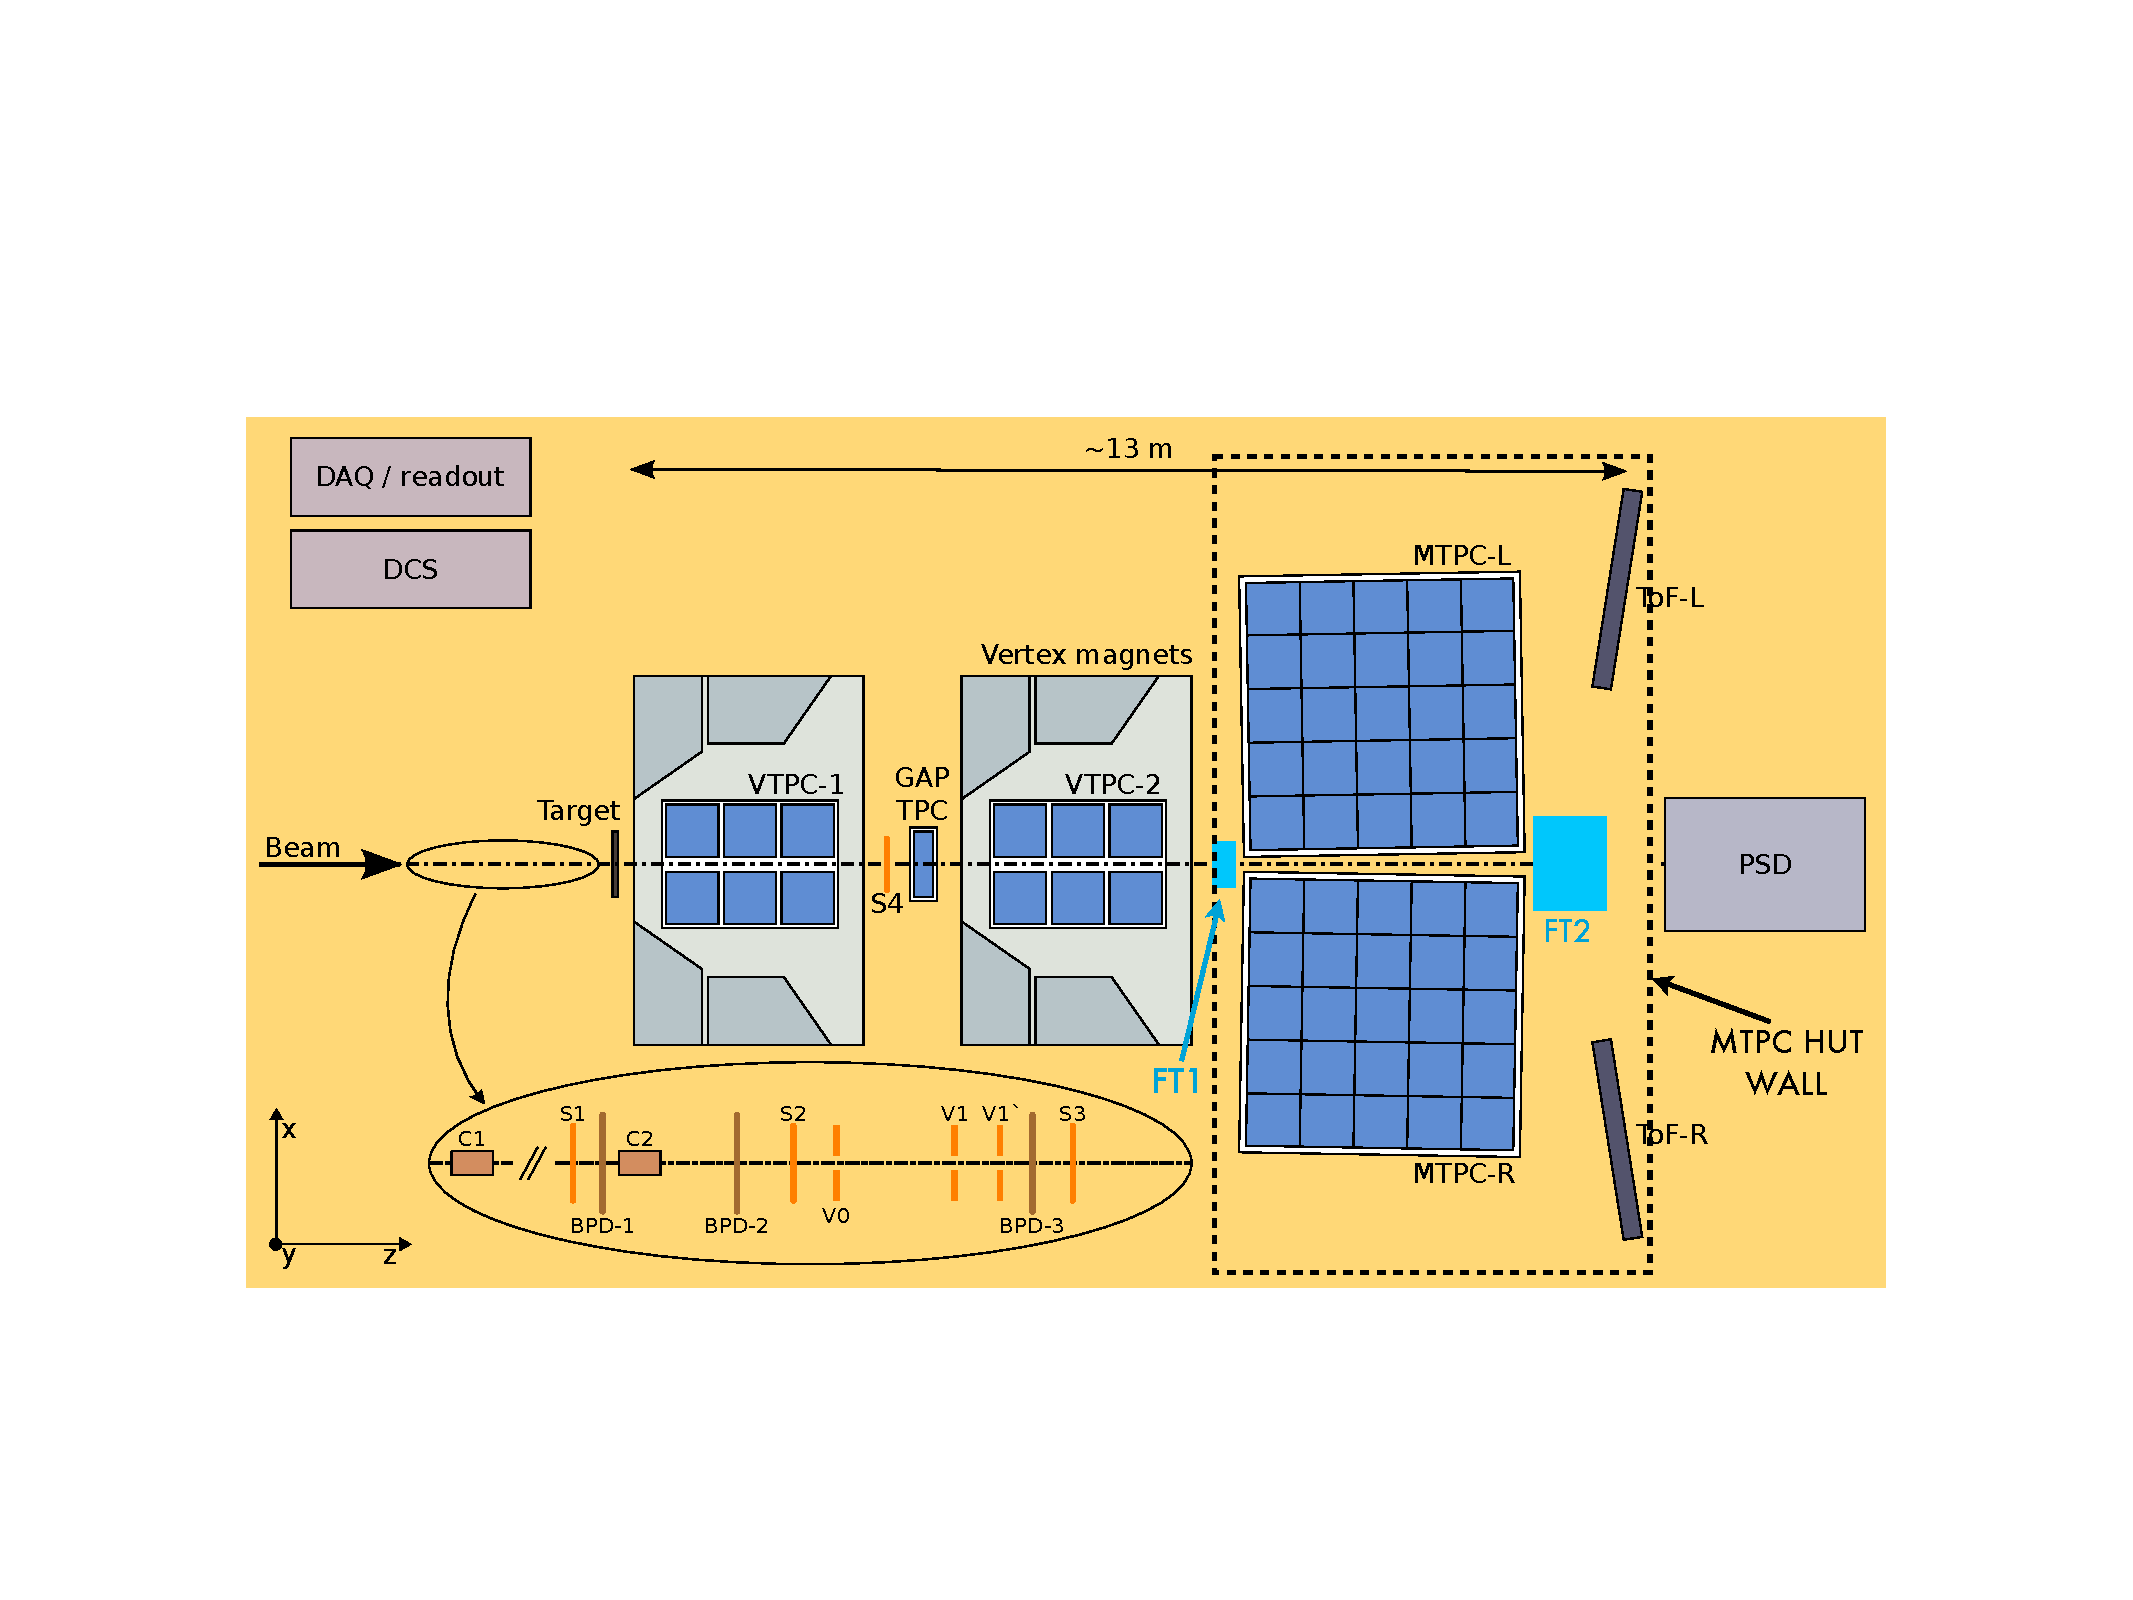
\includegraphics[width=6in]{NA61-PlanView}
\end{cdrfigure}

\begin{cdrfigure}[The 2015 run plan for US-NA61.]{NA61RunPlan}{A table that shows the proposed run plan for 
the US-NA61 data run in the fall of 2015.}
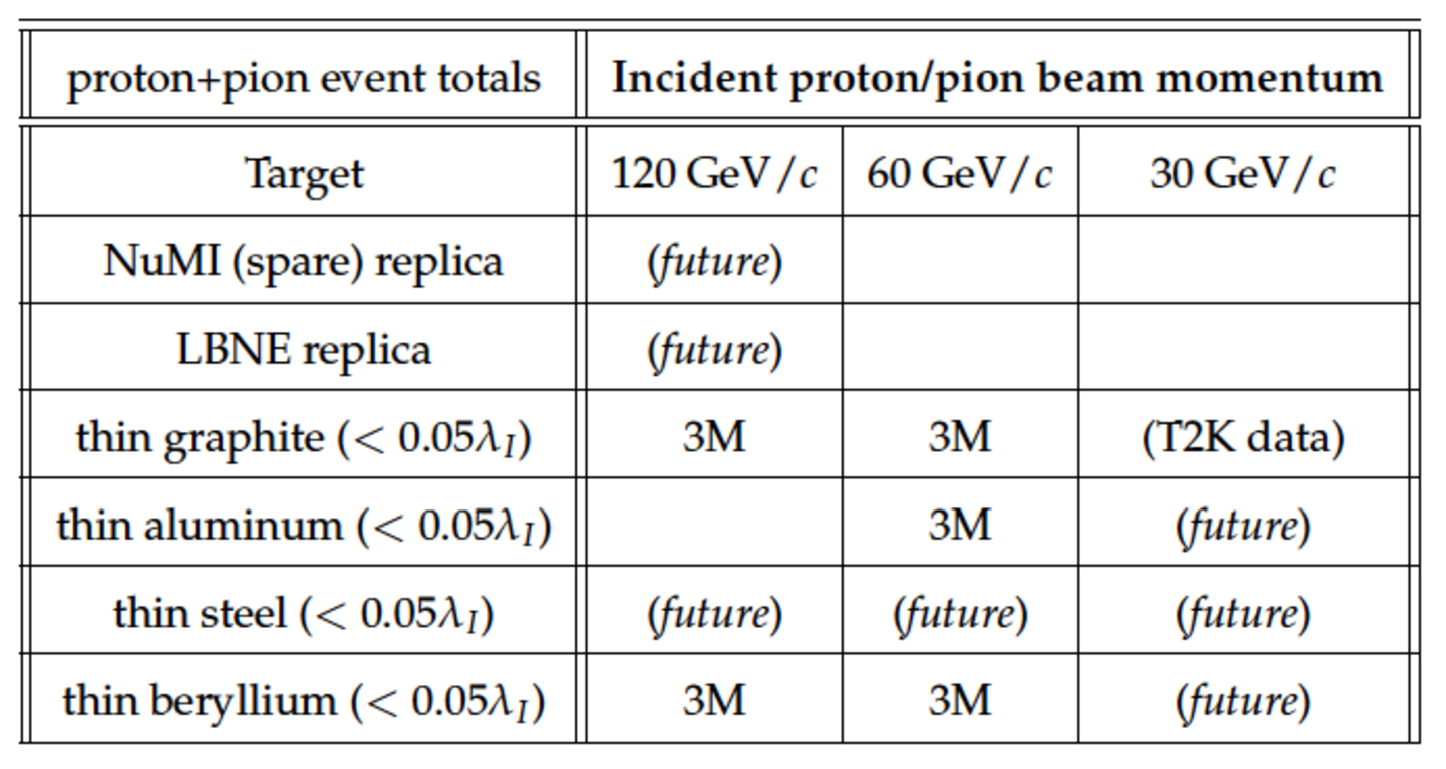
\includegraphics[width=6in]{NA61RunPlan}

\end{cdrfigure}

